\section{Appendix}

% Set supplementary figure numbering
\renewcommand{\thefigure}{S\arabic{figure}}
\setcounter{figure}{0}

\subsection{Software and data availability}
\label{subsection:software_data_availability}

\begin{itemize}

    \item The codebase is implemented in Python using PyTorch and is available at \url{https://github.com/jkbhagatio/mini} under an MIT License for academic use.
    
    \item Example usage of the pipeline along with replication of the paper's results can be found at \url{https://github.com/jkbhagatio/mini/notebooks}.

\end{itemize}

\subsection{On interpretable latents}
\begin{figure}[h]
    \centering
    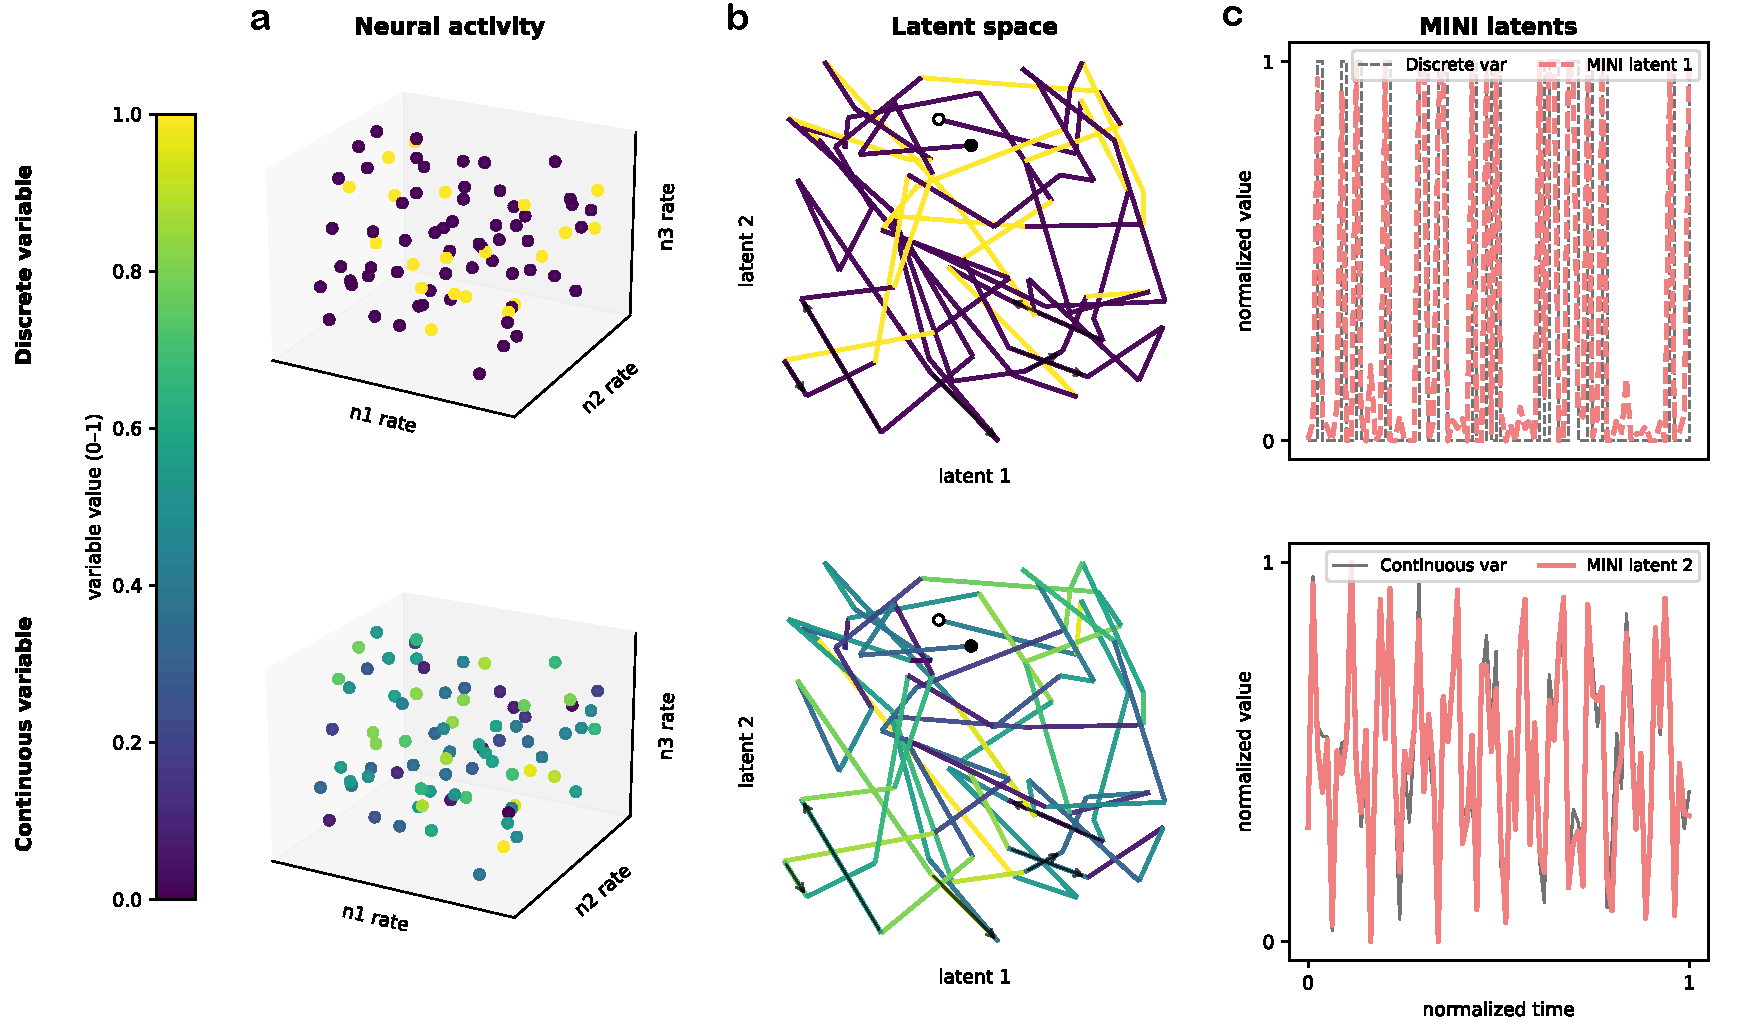
\includegraphics[width=\linewidth]{figures/interpretable_latents_vs_latent_space.pdf}
    \caption{
        \textbf{Interpretable latents in a complex latent space.} \\
        \small This toy example highlights the utility of MINI. The two rows show two different variables (top: discrete; bottom: continuous), each uniquely encoded by the same underlying neural activity made up of three neurons' firing rates. The viridis colorbar shows the variables' values as a function of this neural activity. (\textbf{a}) Each point in the scatterplots represents a moment in time. (\textbf{b}) A projection of this activity into a 2D latent space creates tangled trajectories where variable states (e.g. 'on' and 'off' in the discrete case, and 'high' and 'low' in the continuous case) are not easily distnguished. The start and end points of the trajectories are marked by white and black dots, respectively, while arrows indicate trajectory direction. (\textbf{c}) In contrast to the tangled latent space, MINI finds individual latents corresponding to each variable, demonstrating the potential for improved interpretability of neural representations.
    }
    \label{figure:interpretable_latents_vs_latent_space}
\end{figure}

\subsection{Additional pipeline details}
\label{subsection:additional_pipeline_details}

\subsubsection{Model training details}
\label{subsubsection:model_training_details}

\begin{algorithm}[h!]
\caption{Model training procedure}
\label{algorithm:sdnn_model_training}
\begin{algorithmic}[1]
\State \textbf{Data definitions:}
\State \quad Input neural data: $\mathbf{Y} \in \mathbb{R}^{B \times S_{\text{in}} \times N_{\text{in}}}$ \textsuperscript{(Batch, Sequence length of input data, Input neural units)}
\State \quad Target neural data: $\mathbf{Z} \in \mathbb{R}^{B \times S_{\text{out}} \times N_{\text{out}}}$ \textsuperscript{(Batch, Sequence length of output data, Output neural units)}
\State \textbf{Model definitions:}
\State \quad Encoder: $\mathbf{W}_{\text{enc}} \in \mathbb{R}^{D_{\text{max}} \times S_{\text{in}} \times N_{\text{in}}}$, $\mathbf{b}_{\text{enc}} \in \mathbb{R}^{D_{\text{max}}}$ \textsuperscript{(Hidden layer neurons)}
\State \quad Decoder: $\mathbf{W}_{\text{dec}} \in \mathbb{R}^{S_{\text{out}} \times N_{\text{out}} \times D_{\text{max}}}$, $\mathbf{b}_{\text{dec}} \in \mathbb{R}^{S_{\text{out}} \times N_{\text{out}}}$
\State \quad Transformer block (optional) $\mathbf{\theta_{t}}$: $\{\mathbf{W}_{Q,K,V} \in \mathbb{R}^{D_{\max} \times D_{\max}}, \dots\}$
\State \quad Matryoshka levels: $\mathbf{\{D_l\}_{l=1}^L}$
\State \quad Weights each level's reconstruction loss (optional): $\mathbf{\{\lambda_l\}_{l=1}^L}$
\State \quad Auxiliary loss weight: $\mathbf{\gamma}$
\\
\Procedure{train\_step}{$\mathbf{Y}, \mathbf{Z}$}    
    \Statex \Comment{\textit{--- Forward Pass ---}}
    \State $\mathbf{A} \gets \text{ReLU}(\mathbf{Y}\mathbf{W}_{\text{enc}}^T + \mathbf{b}_{\text{enc}})$ \Comment{Get encoder activations}
    \\
    \If{$S > 1$}
        \State $\mathbf{A} \gets \text{SelfAttention}(\mathbf{A}; \theta_{\text{attn}})$ \Comment{Temporally integrate over latent space}
    \EndIf
    \\
    \State $\mathcal{L}_{\text{recon}} \gets 0$
    \For{$l=1$ to $L$} \Comment{For each level...}
        \State $\hat{\mathbf{A}}_l \gets S_{\text{topk}}(\mathbf{A}_{:, :D_l})$ \Comment{Sparsify latents with batch top-$k$}
        \State $\hat{\mathbf{Z}}_l \gets \text{ReLU}(\hat{\mathbf{A}}_l \mathbf{W}_{\text{dec}, :, :D_l}^T + \mathbf{b}_{\text{dec}})$ \Comment{Reconstruct target (decoder activations)}
        \State $\mathcal{L}_{\text{recon}} \gets \mathcal{L}_{\text{recon}} + \lambda_l \cdot \text{MSLE}(\mathbf{Z}, \hat{\mathbf{Z}}_l)$ \Comment{Get reconstruction loss}
    \EndFor
    
    \Statex \Comment{\textit{--- Auxiliary Loss for Dead Latent Resurrection ---}}
    \State $\mathcal{D} \gets \text{GetDeadLatents}(\mathbf{A})$
    \If{\text{any}($\mathcal{D}$)} \Comment{Only compute if dead latents exist}
        \State $\mathbf{R} \gets \mathbf{Z} - \hat{\mathbf{Z}}_L$ \Comment{Get reconstruction residual}
        \State $\hat{\mathbf{R}} \gets \text{ReLU}((\mathbf{A} \odot \mathcal{D}) \mathbf{W}_{\text{dec}}^T + \mathbf{b}_{\text{dec}})$ \Comment{Reconstruct residual from dead latents}
        \State $\mathcal{L}_{\text{aux}} \gets \text{MSE}(\mathbf{R}, \hat{\mathbf{R}})$ \Comment{Get auxiliary loss}
    \Else
        \State $\mathcal{L}_{\text{aux}} \gets 0$
    \EndIf
    \\
    \State $\mathcal{L}_{\text{total}} \gets \mathcal{L}_{\text{recon}} + \gamma \mathcal{L}_{\text{aux}}$ \Comment{Total loss: reconstruction + auxiliary}

    \Statex \Comment{\textit{--- Backward Pass \& Parameter Update ---}}
    \State $\mathbf{g} \gets \nabla_{\theta} \mathcal{L}_{\text{total}}$ \Comment{Compute gradients, masking $\nabla\mathcal{L}_{\text{aux}}$ to dead latents}
    \State $\theta \gets \text{Update}(\theta, \mathbf{g})$ \Comment{Update model parameters}
\EndProcedure
\end{algorithmic}
\end{algorithm}

Some notes on \nameref{algorithm:sdnn_model_training}:

\paragraph{Dead Latent Resurrection.}
A common failure mode in training SDNNs is "latent death," where dictionary elements cease to activate for any input. We address this with an auxiliary loss designed to revive dead latents. We monitor feature activation frequencies and identify a set of dead latents $\mathcal{D}$. These latents are then trained via an auxiliary MSE loss to reconstruct the residual error of the primary model ($\mathbf{x}_{\text{target}} - \hat{\mathbf{x}}_L$). The gradients from this auxiliary loss are exclusively applied to the parameters of the dead latents, thereby encouraging them to learn useful representations without disrupting the training of active latents.

\subsubsection{Architecture details}
\label{subsubsection:architecture_details}

...

\paragraph{Matryoshka architecture}

- Results with and without Matryoshka architecture.

...

\paragraph{Transformer block for temporal integration of latent space}

- Results with and without transformer block.

...

\begin{itemize}
    
    \item Variant of MSAE as variant of SAE.
    \begin{itemize}
        \item Briefly mention other archs tried: batchTopK winner for sparsity enforcement.
    \end{itemize}
    
    \item In addition to MSAE levels width, briefly mention hyperparameters, expound in Appendix.
    \begin{itemize}
        \item topk per level, loss X per level, seq len for neural data, seq len for latent space used with transformer layer in decoder
    \end{itemize}

\end{itemize}

\begin{itemize}
    \item Training configuration and hyperparameters
    \begin{itemize}
        \item Sparsity / reconstruction trade-off
    \end{itemize}
    \item Results of sweeps
    \item Hardware specs and details from training runs
\end{itemize}

We systematically analyzed the effect of X on reconstruction quality and feature interpretability across all three datasets.

- See ./notes.md

\subsection{Additional Dataset Info}
\label{subsection:additional_dataset_info}

\begin{itemize}
    \item Synthetic dataset
    \begin{itemize}
        \item Exp metadata \& info
        \item Neural data info
        \item Recreation instructions
    \end{itemize}
    
    \item Churchland dataset
    \begin{itemize}
        \item Exp metadata \& info
        \item Neural data info
        \item Access instructions
    \end{itemize}
    
    \item Aeon dataset
    \begin{itemize}
        \item Exp metadata \& info
        \item Neural data info
        \item Recreation instructions
    \end{itemize}
    
    \item Allen dataset
    \begin{itemize}
        \item Exp metadata \& info
        \item Neural data info
        \item Recreation instructions
    \end{itemize}
\end{itemize}

\subsection{Additional results}

\input{appendix/additional_results/additional_results_main}


\subsubsection{Latent comparisons with sparseNMF, t-SNE, and UMAP}
\label{subsubsection:latent_comparisons_traditional}
...

\subsection{Natural mouse spike data in a passive visual task}
\label{subsection:allen_dataset}

...


\subsection{Methods Comparison}

Here we highlight 15 features of neural LVM methods and create a table displaying how MINI and other relevant methods compare against these features.

These features are:
\begin{itemize}
    \item \textit{Requires multimodal data}: Whether the method requires multimodal data (e.g. video data, or various forms of behavioral data, in addition to neural data).
    \item \textit{Requires trial-structured data}: Whether the method requires trial-structured data.
    \item \textit{Supports multimodal data}: Whether the method can incorporate multimodal data, even if not required.
    \item \textit{Supports trial-structured data}: Whether the method can use trial-structured data, even if not required.
    \item \textit{Learns sparse, easily identifiable latents}: Whether the method by default learns sparse, easily identifiable latents.
    \item \textit{Learns hierarchical latents}: Whether the method by default learns latents that are hierarchically organized (e.g. whether the method can learn one latent that corresponds to a particular behavior, and another, sparser latent that corresponds to a sub-behavior of the first)
    \item \textit{Learns temporally precise latents}: Whether the method by default learns latents that are time-locked to neural events at the resolution of the desired event, potentially down to single-spike precision.
    \item \textit{Learns a continuously-valued latent space}: Whether the method by default learns latents that change smoothly as a function of changes in the input neural data.
    \item \textit{Can use temporal dynamics to update the latent space}: Whether the method can use temporal dynamics (e.g. neural data or latent space history) to update the latent space.
    \item \textit{Imposes a prior on the latent space}: Whether the method imposes a predfined structure on the latent space (e.g. geometric constraints like orthogonality of latents, or distributional assumptions like a Gaussian latents).
    \item \textit{Uses nonlinear dynamics}: Whether the method learns latents from  nonlinear neural dynamics.
    \item \textit{Can be used as a generative model}: Whether the method can be used to generate new neural data samples from the learned latent space.
    \item \textit{Enforces neural data reconstruction}: Whether the method needs to perform neural data reconstruction when learning latents.
    \item \textit{Has approximate linear time scaling}: Whether the method has linear time scaling with respect to the number of data points in an example and in the dataset.
    \item \textit{Requires significant hyperparameter tuning}: Whether the method requires significant hyperparameter tuning to learn interpretable latents.
\end{itemize}

Light-green text indicates that the method has an ideal implementation of the feature, while dark-red text indicates a shortcoming.

\newcommand{\goodQual}[1]{\textcolor{green}{#1}}
\newcommand{\badQual}[1]{\textcolor{cb_red}{#1}}
\newcommand*\rot[1]{\rotatebox{90}{\parbox{3cm}{\centering\small #1}}}

\begin{table}[h]
\label{table:method_comparisons}
\centering
\begin{threeparttable}
\setlength{\tabcolsep}{2.5pt}
\renewcommand{\arraystretch}{1.6}
\begin{tabular}{>{\raggedright}m{5cm}|c|c|c|c|c|c|c|c|c|c|}
\toprule
\textbf{Feature} & \rot{\textbf{MINI}*} & \rot{LangevinFlow* \cite{song_2025_langevinflow}} & \rot{CEBRA* \cite{schneider_2023_cebra}} & \rot{ST-NDT \cite{le_2022_stndt}} & \rot{AutoLFADS \cite{keshtkaran_2022_autolfads}} & \rot{UMAP** \cite{mcinnes_2018_umap}} & \rot{t-SNE** \cite{vandermaaten_2008_tsne}} & \rot{sparseNMF** \cite{hoyer_2004_sparsenmf}} & \rot{ICA \cite{comon_1994_ica}} & \rot{PCA \cite{hotelling_1933_pca}} \\
\midrule
Requires multimodal data & \goodQual{No} & \goodQual{No} & \goodQual{No} & \goodQual{No} & \goodQual{No} & \goodQual{No} & \goodQual{No} & \goodQual{No} & \goodQual{No} & \goodQual{No} \\
\hline
Requires trial-structured data & \goodQual{No} & \goodQual{No} & \goodQual{No} & \goodQual{No} & \goodQual{No\textsuperscript{\textasciicircum}} & \goodQual{No} & \goodQual{No} & \goodQual{No} & \goodQual{No} & \goodQual{No} \\
\hline
Supports multimodal data & \badQual{No\textsuperscript{\dag}} & \badQual{No} & \goodQual{Yes} & \badQual{No} & \badQual{No} & \badQual{No} & \badQual{No} & \badQual{No} & \badQual{No} & \badQual{No} \\
\hline
Supports trial-structured data & \goodQual{Yes} & \goodQual{Yes} & \goodQual{Yes} & \goodQual{Yes} & \goodQual{Yes} & \goodQual{Yes} & \goodQual{Yes} & \goodQual{Yes} & \goodQual{Yes} & \goodQual{Yes} \\
\hline
Learns sparse, easily identifiable latents & \goodQual{Yes} & \badQual{No} & \badQual{No} & \badQual{No} & \badQual{No} & \badQual{No} & \badQual{No} & \goodQual{Yes} & \badQual{No} & \badQual{No} \\
\hline
Learns hierarchical latents & \goodQual{Yes} & \badQual{No} & \badQual{No} & \badQual{No} & \badQual{No} & \badQual{No} & \badQual{No} & \badQual{No} & \badQual{No} & \badQual{No} \\
\hline
Learns temporally precise latents & \goodQual{Yes} & \goodQual{Yes} & \goodQual{Yes} & \goodQual{Yes} & \goodQual{Yes} & \badQual{No} & \badQual{No} & \goodQual{Yes} & \badQual{No} & \badQual{No} \\
\hline
Learns a continuously-valued latent space & \badQual{No\textsuperscript{\ddag}} & \goodQual{Yes} & \goodQual{Yes} & \goodQual{Yes} & \goodQual{Yes} & \goodQual{Yes} & \goodQual{Yes} & \badQual{No\textsuperscript{\ddag}} & \goodQual{Yes} & \goodQual{Yes} \\
\hline
Can use temporal dynamics to update the latent space & \goodQual{Yes} & \goodQual{Yes} & \goodQual{Yes} & \goodQual{Yes} & \goodQual{Yes} & \badQual{No} & \badQual{No} & \badQual{No} & \badQual{No} & \badQual{No} \\
\hline
Imposes a prior on the latent space & \goodQual{No} & \badQual{Yes} & \goodQual{No} & \goodQual{No} & \badQual{Yes} & \goodQual{No} & \goodQual{No} & \goodQual{No} & \badQual{Yes} & \badQual{Yes} \\
\hline
Uses nonlinear dynamics & \goodQual{Yes} & \goodQual{Yes} & \goodQual{Yes} & \goodQual{Yes} & \goodQual{Yes} & \badQual{No} & \badQual{No} & \badQual{No} & \badQual{No} & \badQual{No} \\
\hline
Can be used as a generative model & \goodQual{Yes} & \goodQual{Yes} & \goodQual{Yes} & \goodQual{Yes} & \goodQual{Yes} & \badQual{No} & \badQual{No} & \badQual{No} & \badQual{No} & \badQual{No} \\
\hline
Enforces neural data reconstruction & \badQual{Yes} & \badQual{Yes} & \goodQual{No} & \badQual{Yes} & \badQual{Yes} & \goodQual{No} & \goodQual{No} & \badQual{Yes} & \goodQual{No} & \goodQual{No} \\
\hline
Has approximate linear time scaling & \goodQual{Yes\textsuperscript{\#}} & \badQual{No} & \goodQual{Yes} & \badQual{No} & \badQual{No} & \goodQual{Yes} & \badQual{No} & \badQual{No} & \goodQual{Yes} & \goodQual{Yes} \\
\hline
Requires significant hyperparameter tuning & \badQual{Yes} & \badQual{Yes} & \badQual{Yes} & \badQual{Yes} & \badQual{Yes} & \badQual{Yes} & \badQual{Yes} & \badQual{Yes} & \goodQual{No} & \goodQual{No} \\
\bottomrule
\end{tabular}
\caption{\centering Comparison of MINI with other neural LVM methods.}
\begin{tablenotes}[flushleft]
\footnotesize
\item *: Latent comparison visualized in \nameref{section:results}
\item **: Latent comparison visualized in \nameref{subsubsection:latent_comparisons_traditional}
\item \textsuperscript{\dag}: Not a fundamental limitation -- could be added as a feature
\item \textsuperscript{\ddag}: Enforced sparsity can cause step-like jumps in the data-to-latents mapping
\item \textsuperscript{\#}: In the standard implementation, without a transformer layer in the decoder
\item \textsuperscript{\textasciicircum}: Can bin data to create ``pseudo''-trials
\end{tablenotes}
\end{threeparttable}
\end{table}

\newpage

% TODO: review and add MINI!
Below we provide a brief justification of the table entries.

\begin{itemize}
\item \textbf{Requires multimodal data}
    \begin{itemize}
    \item \textit{PCA} — No. Classic PCA factorizes a single data matrix and does not require paired behavioral or other modalities.
    \item \textit{sparseNMF} — No. NMF with sparsity constraints operates on one non-negative matrix; no second modality is needed.
    \item \textit{LangevinFlow} — No. It's a sequential VAE for neural population dynamics; it models spikes/rates without needing aligned behavioral inputs.
    \item \textit{CEBRA} — No. CEBRA supports supervised multimodal training, but it also has an unsupervised "label-free" mode on neural-only data.
    \item \textit{ST-NDT} — No. The model is trained on spike counts/rates and does not intrinsically require a second modality.
    \item \textit{AutoLFADS} — No. AutoLFADS infers latent dynamics from neural data alone (behavior is often used only for downstream decoding).
    \end{itemize}

\item \textbf{Requires trial-structured data}
    \begin{itemize}
    \item \textit{PCA} — No. Matrix decomposition does not assume trials.
    \item \textit{sparseNMF} — No. Standard NMF does not require trial segmentation.
    \item \textit{LangevinFlow} — No. It is defined on continuous time series and can be trained on long, unsegmented recordings.
    \item \textit{CEBRA} — No. CEBRA works across sessions and continuous recordings; its sampling scheme does not require explicit trial boundaries.
    \item \textit{ST-NDT} — No. Although many datasets are organized as trials, ST-NDT's masked-modeling objective applies to continuous sequences as well.
    \item \textit{AutoLFADS} — No (footnote in your table). AutoLFADS has been used on continuous data and can be applied without true trial structure (e.g., via windowing/pseudo-trials).
    \end{itemize}

\item \textbf{Supports multimodal data}
    \begin{itemize}
    \item \textit{PCA} — No. While you can concatenate features, PCA is not designed for cross-modal alignment or contrastive objectives.
    \item \textit{sparseNMF} — No. The basic objective reconstructs a single non-negative matrix, not joint modalities.
    \item \textit{LangevinFlow} — No. The described model targets neural dynamics; multimodal coupling is not a core feature.
    \item \textit{CEBRA} — Yes. It explicitly supports joint neural–behavioral training (supervised) as well as label-free training, enabling cross-modal embeddings.
    \item \textit{ST-NDT} — No. It models neural population activity; multimodal alignment is not part of the method.
    \item \textit{AutoLFADS} — No. The VAE reconstructs neural observations; other modalities are typically used only for evaluation/decoding.
    \end{itemize}

\item \textbf{Supports trial-structured data}
    \begin{itemize}
    \item \textit{PCA / sparseNMF / LangevinFlow / CEBRA / ST-NDT / AutoLFADS} — Yes. All can be applied to trialized datasets (matrix rows/time bins per trial; masking across trial windows; or VAE sequences per trial).
    \end{itemize}

\item \textbf{Learns sparse, easily identifiable latents}
    \begin{itemize}
    \item \textit{PCA} — No. Principal components are dense linear combinations and typically not parts-based or sparse without additional penalties.
    \item \textit{sparseNMF} — Yes. The objective adds explicit sparsity constraints, producing parts-based, interpretable components and sparse activations.
    \item \textit{LangevinFlow} — No. The sequential VAE uses continuous latent dynamics without an inherent sparsity/parts constraint.
    \item \textit{CEBRA} — No. The contrastive embedding is learned by an encoder; there's no explicit sparsity/parts prior on latent coordinates.
    \item \textit{ST-NDT} — No. Transformer representations/rate outputs are not designed to be sparse components.
    \item \textit{AutoLFADS} — No. LFADS/AutoLFADS learn dense low-dimensional factors unless additional sparsity regularizers are added.
    \end{itemize}

\item \textbf{Learns hierarchical latents}
    \begin{itemize}
    \item \textit{PCA / sparseNMF / LangevinFlow / CEBRA / ST-NDT / AutoLFADS} — No. None of these methods impose a hierarchical/nesting constraint over features by default. (See their objectives/architectures; no nested-feature prior is specified.)
    \end{itemize}

\item \textbf{Learns temporally precise latents}
    \begin{itemize}
    \item \textit{PCA} — No. Components are static projections with no temporal state update.
    \item \textit{sparseNMF} — Yes (per your table). When applied to time-binned data (or with sequence/convolutional extensions), NMF can isolate time-localized motifs, yielding temporally sharp activations even without a dynamics model.
    \item \textit{LangevinFlow} — Yes. Latents evolve via an underdamped Langevin SDE inside a sequential VAE, giving fine-grained temporal trajectories.
    \item \textit{CEBRA} — Yes. Its time-aware sampling scheme shapes embeddings to be consistent across nearby time points, supporting temporally resolved latents/decoding.
    \item \textit{ST-NDT} — Yes. It infers single-trial firing rates at each time bin using spatiotemporal attention and masked reconstruction.
    \item \textit{AutoLFADS} — Yes. AutoLFADS yields high-time-resolution single-trial rate estimates.
    \end{itemize}

\item \textbf{Learns a continuously-valued latent space}
    \begin{itemize}
    \item \textit{PCA} — Yes. Continuous linear coordinates (principal components).
    \item \textit{sparseNMF} — No (per your table). In practice, sparsity constraints drive near-binary/parts-activation patterns rather than a smooth, unconstrained continuous code.
    \item \textit{LangevinFlow} — Yes. Latents follow continuous SDE dynamics.
    \item \textit{CEBRA} — Yes. Encoded embeddings are continuous vectors optimized by a contrastive loss.
    \item \textit{ST-NDT} — Yes. The model predicts continuous firing-rate trajectories (with spikes modeled as Poisson draws from those rates).
    \item \textit{AutoLFADS} — Yes. LFADS/AutoLFADS learn continuous latent factors/generator states.
    \end{itemize}

\item \textbf{Can use temporal dynamics to update the latent space}
    \begin{itemize}
    \item \textit{PCA} — No. No state evolution; projections are static.
    \item \textit{sparseNMF} — No. Standard NMF has no transition prior/dynamics.
    \item \textit{LangevinFlow} — Yes. Latents evolve via Langevin dynamics between time steps.
    \item \textit{CEBRA} — Yes. The training pairs/sampling function incorporate temporal neighborhoods, effectively using time to shape the embedding.
    \item \textit{ST-NDT} — Yes. Self-attention across time learns temporal dependencies and updates inferred rates accordingly.
    \item \textit{AutoLFADS} — Yes. The generator RNN (and inferred inputs) explicitly model latent temporal evolution.
    \end{itemize}

\item \textbf{Imposes a prior on the latent space}
    \begin{itemize}
    \item \textit{PCA} — Yes. In the PPCA view, latents have an isotropic Gaussian prior; PCA emerges as ML under this generative model.
    \item \textit{sparseNMF} — No. It is an optimization with non-negativity/sparsity constraints, not a probabilistic latent prior.
    \item \textit{LangevinFlow} — Yes. The latent time evolution is governed by a physical prior (underdamped Langevin SDE/potential), combined with a VAE likelihood.
    \item \textit{CEBRA} — No. It uses a contrastive objective; there's no explicit generative prior over latents.
    \item \textit{ST-NDT} — No. Training is via masked reconstruction/contrastive loss, not a latent prior.
    \item \textit{AutoLFADS} — Yes. As a VAE, it places priors over latent initial conditions/inputs/dynamics.
    \end{itemize}

\item \textbf{Uses nonlinear dynamics}
    \begin{itemize}
    \item \textit{PCA} — No. Linear projection model.
    \item \textit{sparseNMF} — No. Linear parts-based factorization.
    \item \textit{LangevinFlow} — Yes. Nonlinear latent dynamics via learned potential and stochastic forces.
    \item \textit{CEBRA} — Yes. Nonlinear encoder network learns the embedding.
    \item \textit{ST-NDT} — Yes. Transformer attention is a nonlinear mapping.
    \item \textit{AutoLFADS} — Yes. Generator RNN defines nonlinear latent dynamics.
    \end{itemize}

\item \textbf{Can be used as a generative model}
    \begin{itemize}
    \item \textit{PCA} — No. PCA is not a generative model (absent the PPCA extension's explicit likelihood).
    \item \textit{sparseNMF} — No. Standard NMF reconstructs the data matrix but is not typically used for sampling new sequences.
    \item \textit{LangevinFlow} — Yes. It is a VAE with Langevin latent dynamics, enabling simulation/decoding from the learned generative process.
    \item \textit{CEBRA} — No. The authors emphasize that CEBRA is not a generative model.
    \item \textit{ST-NDT} — Yes. Given inferred rate trajectories and a Poisson observation model, one can generate spikes by sampling from the inhomogeneous Poisson with the model's rates.
    \item \textit{AutoLFADS} — Yes. LFADS/AutoLFADS are VAEs that generate neural activity via a latent dynamical system and observation model.
    \end{itemize}

\item \textbf{Enforces neural data reconstruction}
    \begin{itemize}
    \item \textit{PCA} — Yes. Minimizes reconstruction error under a rank constraint (equivalently maximizes variance explained).
    \item \textit{sparseNMF} — Yes. Objective reconstructs the input with non-negativity and sparsity penalties.
    \item \textit{LangevinFlow} — Yes. Trained via an ELBO with a likelihood term that reconstructs neural observations from latents.
    \item \textit{CEBRA} — No. It optimizes a contrastive loss rather than a reconstruction loss.
    \item \textit{ST-NDT} — Yes. Uses masked modeling (reconstructing held-out bins) and an auxiliary contrastive loss.
    \item \textit{AutoLFADS} — Yes. As a VAE, it reconstructs spikes/rates through the decoder likelihood.
    \end{itemize}

\item \textbf{Has approximate linear time scaling}
    \begin{itemize}
    \item \textit{PCA} — Yes. With randomized/incremental PCA, computation scales near-linearly with the number of samples.
    \item \textit{sparseNMF} — No. Iterative multiplicative/gradient updates with sparsity constraints can be comparatively slow and require many passes/hyperparameters.
    \item \textit{LangevinFlow} — Yes. Mini-batch VAE training scales roughly linearly in dataset size. (Model is designed for large neural recordings.)
    \item \textit{CEBRA} — Yes. Contrastive encoders trained with mini-batches scale well to large, multi-session datasets.
    \item \textit{ST-NDT} — No. Spatiotemporal self-attention is quadratic in sequence length (and also attends across neurons), so compute grows super-linearly.
    \item \textit{AutoLFADS} — No. Although each SGD step is linear in batch size, the heavy hyperparameter search (PBT) makes effective compute scale poorly.
    \end{itemize}

\item \textbf{Requires significant hyperparameter tuning}
    \begin{itemize}
    \item \textit{PCA} — No. Essentially parameter-free aside from the chosen rank.
    \item \textit{sparseNMF} — Yes. You must pick rank and sparsity levels; performance depends strongly on these choices.
    \item \textit{LangevinFlow} — Yes. Sequential VAE with SDE dynamics introduces choices for latent dimensionality, dynamics hyperparameters, and optimizer settings.
    \item \textit{CEBRA} — Yes. Results depend on encoder architecture, temperature, sampling function, supervision mode, etc.
    \item \textit{ST-NDT} — Yes. Transformer depth/width, attention configuration, masking schedule, and losses require tuning.
    \item \textit{AutoLFADS} — Yes. The method is explicitly built around automated hyperparameter search (population-based training).
    \end{itemize}
\end{itemize}
